\chapter{Experimentación y evaluación}


%-----------------------------------------------
% 5.1 Scientific workflows
%-----------------------------------------------
\section{Experimentos computacionales}\label{s5.1}

Para validar nuestra propuesta y como ésta puede aplicada en el contexto de workflows científicos, se ha selecciona un subconjunto de workflows y WMSs. 
El subconjunto ha sido seleccionado bajo a los criterio de: nivel de utilización de WMSs, lenguaje utilizados, y disponibilidad de los materiales. 
Estos materiales incluye los datos de ingresos que permiten reproducir de forma completa el workflow. y documentación, resultados o anotaciones que nos permitan comparar los resultados de nuestro ambientes.


Para cada WMS, he construimos una imagen estándar. En consecuencia, un investigador puede importar esta imagen e instalar los componentes de software relacionados con el flujo de trabajo.
Esto se puede conseguir utilizando la instrucción FROM de Dockerfile. Por ejemplo, el flujo de trabajo de SoyKB utiliza el gestor de flujo de trabajo: Pegasus. Por lo tanto, la imagen SoyKb importa la imagen Pegasus.

Para entender los requisitos del flujo de trabajo, nosotros inspeccionamos la documentación del flujo de trabajo disponible y las anotaciones generadas por WICUS.
En caso que el WMSs no distribuya su software utilizando Docker hemos construidos las imágenes necesarias, los archivos necesarios son las configuraciones y el DeploymentPlan (Dockerfile). Estos archivos están disponibles en nuestros repositorios para cada flujo de trabajo. \footnote{https://github.com/dockerpedia}.
Además, cada DeploymentFile incluye información sobre el contenedor utilizando el estándar de la Open Container Initiative \footnote{\url{https://www.opencontainers.org/}}. 


\subsection{Pegasus}


Pegasus~\cite{} es un WMS capaz de gestionar flujos de trabajo compuestos por millones de tareas, registrando datos sobre la ejecución y resultados intermedios. 
Cuando se producen errores, Pegasus intenta recuperarse cuando es posible reintentando tareas, reintentando todo el flujo de trabajo, proporcionando puntos de control a nivel de flujo de trabajo, re-mapeando partes del flujo de trabajo, probando fuentes de datos alternativas para la puesta a disposición de los datos y, cuando todo lo demás falla, proporcionando un flujo de trabajo de rescate que contiene sólo una descripción del trabajo que queda por hacer. Limpia el almacenamiento a medida que se ejecuta el flujo de trabajo, de modo que los flujos de trabajo de datos intensivos tengan suficiente espacio para ejecutarse en recursos limitados por el almacenamiento]. Pegasus lleva un registro de lo que se ha hecho (procedencia), incluyendo las ubicaciones de los datos utilizados y producidos, y qué software se utilizó con qué parámetros.
Pegasus lee las descripciones del flujo de trabajo de los archivos DAX. El término DAX" es la abreviatura de "Directed Acyclic Graph in XML". DAX es un formato de archivo XML que tiene sintaxis para expresar trabajos, argumentos, archivos y dependencias. Para crear un DAX es necesario escribir código para un generador de DAX. 
Pegasus opcionalmente utiliza en HTCondor como administrador de tareas. Por lo tanto, construimos dos versión para la imagen de Pegasus; una versión tiene instalado el paquete condor y otra sin él. La justificación de decisión recae en permitir a los científicos utilizar una imagen simple si es necesario.
El paquete Pegasus ha sido obtenido del repositorio oficial~\footnote{http://download.pegasus.isi.edu/wms/download/debian}.


Los principales requisitos de pegasus son: openssh-server, condor y JAVA (la versión Java depende de la versión pegasus).


Las imágenes se encuentran disponibles en DockerHub~\footnote{\url{https://hub.docker.com/r/dockerpedia/pegasus_workflow_images/}}



\subsection{SoyKB}

%todo: cambiar es copia
SoyKB (Soybean Knowledge Base)
El workflow SoyKB (Soybean Knowledge Base) (Joshi et al., 2014a,b) es una pipeline de genómas que re-secuencia las líneas de germoplasma de soya seleccionadas para rasgos deseables tales como aceite, proteína, resistencia a nematoda del quiste de soja, resistencia al estrés y arquitectura del sistema radicular. El flujo de trabajo (Figura 6.5) implementa una pipeline de identificación y análisis de Polimorfismo de Nucleótido Único (SNP) e inyección/deliminación (indel) utilizando el llamador de haplotipo GATK86 y un genoma de referencia de soja.

El flujo de trabajo analiza muestras en paralelo para alinearlas con el genoma de referencia, desduplicar los datos, identificar indel y SNPs, y fusionar y filtrar los resultados.

Los resultados se utilizan luego para estudios de asociación de todo el genoma (GWAS) y análisis de genotipo a fenotipo. La instancia de flujo de trabajo utilizada en este proceso de evaluación se basa en un conjunto de datos de muestra que requiere menos memoria que un flujo de trabajo de producción a escala completa, sin embargo, lleva a cabo el mismo proceso y requiere los mismos componentes de software.

%fin de copia

Los componentes de software utilizados por SoyKB son comp




\subsection{Montage}

The Montage workflow (Berriman et al., 2004) was created by the NASA Infrared Processing and Analysis Center (IPAC) as an open source toolkit that can be used to generate custom mosaics of astronomical images in the Flexible Image Transport System (FITS) format. In a Montage workflow, the geometry of the output mosaic is calculated from the input images. The inputs are then re-projected to have the same spatial scale and rotation, the background emissions in the images are corrected to have a uniform level, and the re-projected, corrected images are co-added to form the output mosaic.


Figure 6.2 illustrates a small Montage workflow, depicting the different transforma- tions performed in it, being each node related to a different binary software component. Therefore, in this experiment, 9 Montage software components were identified, which are linked to the generated requirements. Even though they were not specified in the definition of the workflow, another two components were also detected and included as dependencies in the software catalog: mDiffFit depends on the mDiff and mFitPlane components, as depicted in figure 6.7.




\section{Displey4py}

Displey4py ~\cite{} es una biblioteca Python para describir flujos de trabajo. Describe flujos de trabajo abstractos para aplicaciones intensivas, que luego se traducen y ejecutan en plataformas distribuidas (por ejemplo, Apache Storm, clusters MPI, etc.).
El paquete dispel4py ha sido obtenido del repositorio oficial. Las imágenes están disponibles en DockerHub~\footnote{\url{https://hub.docker.com/r/dockerpedia/internal_extinction/}}. Para la instalación el paquete, utilizamos Conda, un gestor de paquetes, dependencias y entornos para cualquier lenguaje Python, R, Ruby,
Lua, Scala, Java, JavaScript, C/ C\+\+, FORTRAN y es ampliamente utilizado en entornos de \textit{Jupyter notebook}. Para asegurar la versión de los paquetes que se instalarán, incluimos la lista completa de los paquetes instalados en el repositorio GitHub

\subsection{Internal extinction}

Taking as entry point a Virtual Observatory (VO) service, published under the In- ternational Virtual Observatory Alliance91 (IVOA) specification, the int\_ext workflow (Filgueira et al., 2015) calculates the internal extinction factor of galaxies. Using the galaxy catalog provided by AMIGA92, this workflow, which has been also implemented using Taverna, calculates this property, which represents the dust extinction within a galaxy and is used as a correction factor for analyzing its optical luminosity.
Figure 6.9 shows the main structure of the workflow, developed as a pipeline com- posed by four different PEs. The process starts by reading the input coordinates con- taining the right ascension and declination values of 1051 galaxies. Then, a VO service is queried for each of these galaxies using the ascension and declination values. The results of these queries are filtered in the third step, removing those that do not correspond to the morphological type and apparent flattening features of the studied galaxies. Finally, the last PE calculates the internal extinction value of each galaxy.

\subsection{Seismic Ambient Noise Cross-Correlation}

The Seismic Ambient Noise Cross-Correlation workflow (also referred as xcorr) (Fil- guiera et al., 2014) was developed as part of the VERCE project96 for processing and cross-correlating time series (traces) from seismic stations. These traces include many geophysical properties, such as wave velocities or event rates, which have to be processed in nearly real-time for hazard forecasting.

\section{WINGS}

WINGS es un sistema de flujo de trabajo semántico que ayuda a los científicos en el diseño de experimentos computacionales. Un experimento computacional especifica cómo deben ser procesados los conjuntos de datos seleccionados por una serie de componentes de software en una configuración particular.
Los principales requisitos de pegasus son: Docker, Tomcat y JAVA (la versión Java depende de la versión pegasus).
WINGS a diferencia de los otros sistemas de workflows utiliza imágenes Docker para su distribución. La imagen de sistema se encuentra disponible en \footnote{\url{https://hub.docker.com/r/dockerpedia/wings-docker/}}



\subsection{MODFLOW-NWT}

MODFLOW es el modelo hidrológico modular del USGS. MODFLOW se considera una norma internacional para simular y predecir las condiciones de las aguas subterráneas y las interacciones entre las aguas subterráneas y las aguas superficiales.

El USGS MODFLOW-NWT es una formulación de Newton-Raphson para MODFLOW-2005 para mejorar la solución de problemas de flujo de aguas subterráneas no confinadas. MODFLOW-NWT es un programa independiente destinado a resolver problemas de secado y rehumectación de las no linealidades de la ecuación de flujo de agua subterránea no confinada.


\begin{figure}[t]
\centering
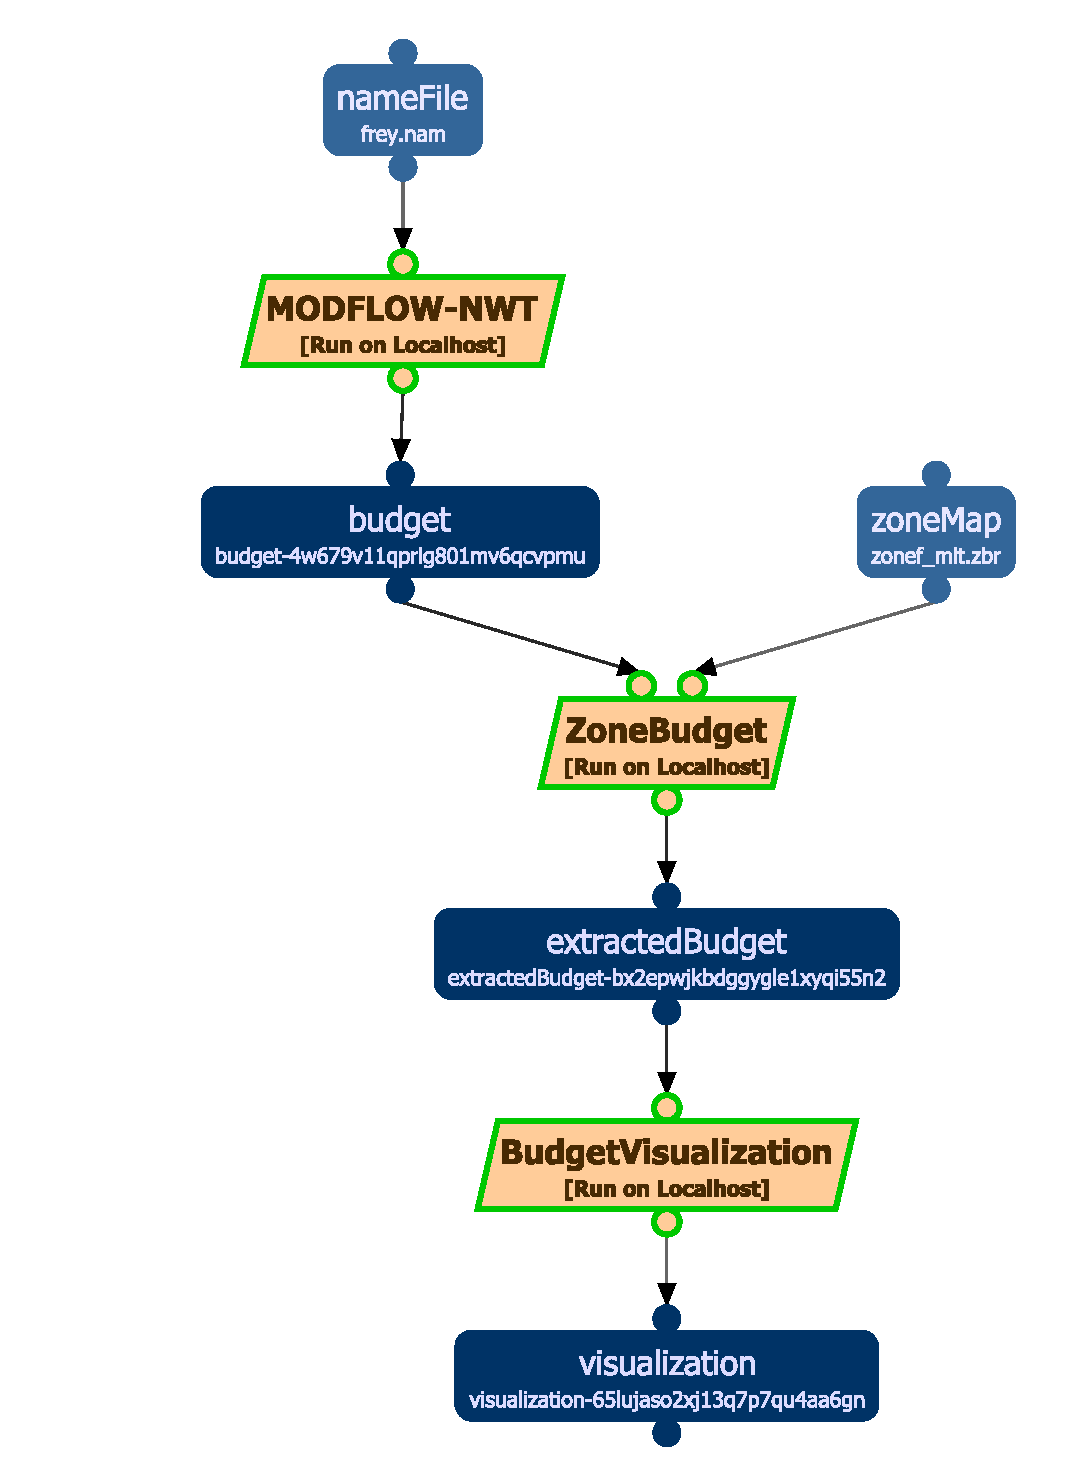
\includegraphics[width=0.6\textwidth]{Figures/usgs-modflow-nwt}
\caption{Figure caption.}\label{fig:modflow}
\end{figure}


\ref{fig:modflow} muestra la estructura principal del worlflow, desarrollado con pipeline compuesto por tres pasos. El proceso inicia leyendo el modelo a utilizar. Luego, el archivo de zona se usa para especificar arreglos de zonas que pueden usarse para especificar las celdas en una variable de capa que están asociadas con un parámetro.

\begin{figure*}[]
    \centering
    \begin{subfigure}[b]{\textwidth}
         \centering
         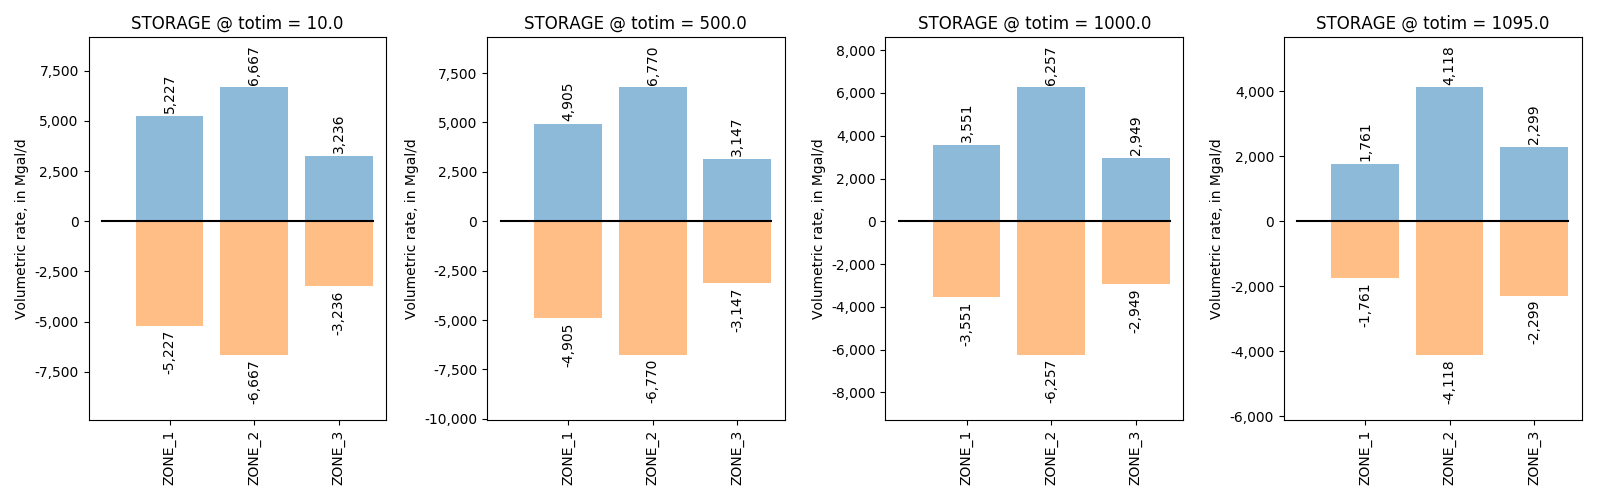
\includegraphics[width=\textwidth]{Figures/viz-original}
         \caption{Resultados originales entregados por el Information Sciences Institute}
         \label{fig:modflow-}
     \end{subfigure}
	
	    \begin{subfigure}[b]{\textwidth}
         \centering
         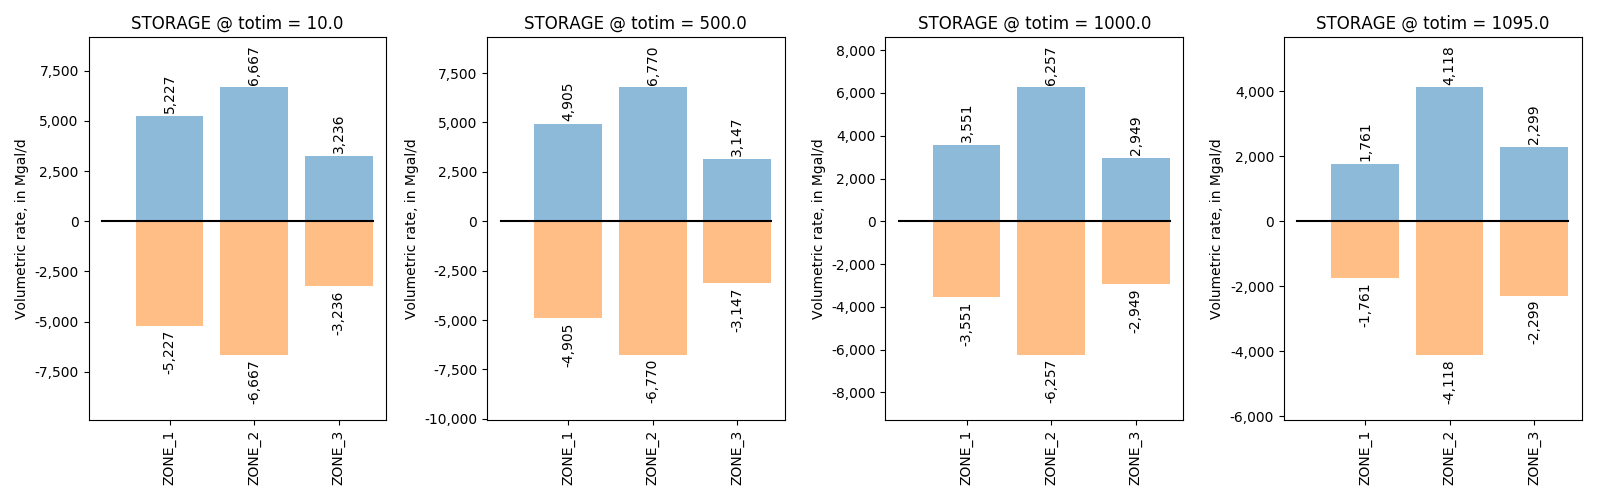
\includegraphics[width=\textwidth]{Figures/viz-original}
         \caption{Resultados reproducidos por nuestra propuesta}
         \label{fig:pegasus48}
     \end{subfigure}
        \caption{Los resultados obtenidos con el nuevo ambiente son iguales}
        \label{fig:dependencies-graph}
\end{figure*}




%----------------------------------
% containerization 
%%%%%%%%%%%%%%%%
\section{Experimentos computacionales}







%-----------------------------------------------
% 5.2 Physical conservation
%-----------------------------------------------
\subsection{Physical conservation}\label{s5.2}

Dado que publicamos las imágenes con su correspondiente Dockerfile, cualquier usuario puede inspeccionarlas y mejorarlas. Las imágenes puede ser encontradas en DockerHub \footnote{https://hub.docker.com/u/dockerpedia/}. 

Para evaluar la conservación física utilizamos tres proveedores diferentes: DigitalOcean, Google Cloud y un local. La figura de \ref{image-env} presenta una descripción de las características de los ambientes    

\begin{table}[]
\begin{tabular}{|l|l|l|l|}
\hline
Resource   & Digital Ocean & Google Compute & Local     \\ \hline
RAM (GB)   & 8             & 8              & 4         \\ \hline
Disk (GB)  & 100           & 100            & 70        \\ \hline
CPU (GHz)  &               &                &           \\ \hline
CPU (Arch) & 64            & 64             & 64        \\ \hline
OS         & Centos 7      & Debian 9       & Fedora 27 \\ \hline
\end{tabular}
\caption{Image appliances characteristics.}
\label{image-env}
\end{table}

El ambiente debe tener instalado Docker, la información del manifiesto de la imagen de Docker describe la versión de Docker necesaria. Sin embargo, Docker asegura idempontencia para los ambientes CentOS7, Debian 10/9/8/7.7, Fedora 26/27/28, Ubuntu 14.04/16.06/18.04, Windows 10, macOS El Capitan 10.11 o nuevas versiones. El proceso de instalación puede ser encontrado en la documentación oficial \url{https://docs.docker.com/install/}

Cada imagen de Docker tiene archivo README con las instrucciones para correr el experimento. Las figuras \ref{lst:1,lst:2,lst3}  muestran los pasos necesarios para correr el experimento computacional. 

Para correr el experimento y descargar la imagen

\begin{lstlisting}[caption={Descarga y correr la imagen disponible en DockerHub mosorio/pegasus\_workflow\_images:soykb},label={lst:1},language=bash]
docker run -d --rm -it --name soybean \
 mosorio/pegasus_workflow_images:soykb
\end{lstlisting}

Luego, el usuario debe entrar al container. El usuario puede confirmar que se encuentra dentro del container por el cambio de símbolo de la terminal  (prompt).

\begin{lstlisting}[caption={Entrar al ambiente computacional utilizando bash},label={lst:2},language=bash]
root@docker-instance:~# docker exec \
-ti -u workflow:workflow soybean bash
workflow@a0f861e6fbc4:~ 
\end{lstlisting}

Finalmente, correr el workflow. 

\begin{lstlisting}[caption={Run the workflow},label={lst:3},language=bash]
workflow@a0f861e6fbc4:~/soykb \
./workflow-generator --exec-env distributed	
\end{lstlisting}

Para evaluar si las imágenes Docker son livianas y almacenables, nosotros construimos dos imágenes, una utilizando Docker y otra utilizando máquinas virtuales. La imagen de Docker se construye bajo nuestro enfoque y la imagen de la máquina virtual basada en el trabajo de ~\cite{santana2017reproducibility}. Luego comparamos el uso de disco de ambas.



%-------------------------------------------
% Logical conservation
%-----------------------------------------------
\subsection{Conservación lógica}\label{s5.3}

A través de las anotaciones realizadas, buscamos construir un ambiente computacional similar que permita reproducir la ejecución del workflow. 

Anotamos los flujos de trabajo con nuestra herramienta, las anotaciones están agrupadas por: pasos de construcción y componentes de software. 

Para evaluar la calidad de las anotaciones utilizamos dos experimentos.

\begin{itemize}
	\item Reproducir el ambiente utilizando los pasos de construcción representados por DeploymentPlan
	\item Detectar las similitudes y diferencias entre dos ambientes computacionales usando distintas versiones de la distribución Linux.
\end{itemize}

Para obtener las anotaciones, proponemos usar Clair y construir un sistema de anotador. La figura \ref{fig:arch} muestra los pasos principales del sistema.


\begin{figure*}[t]
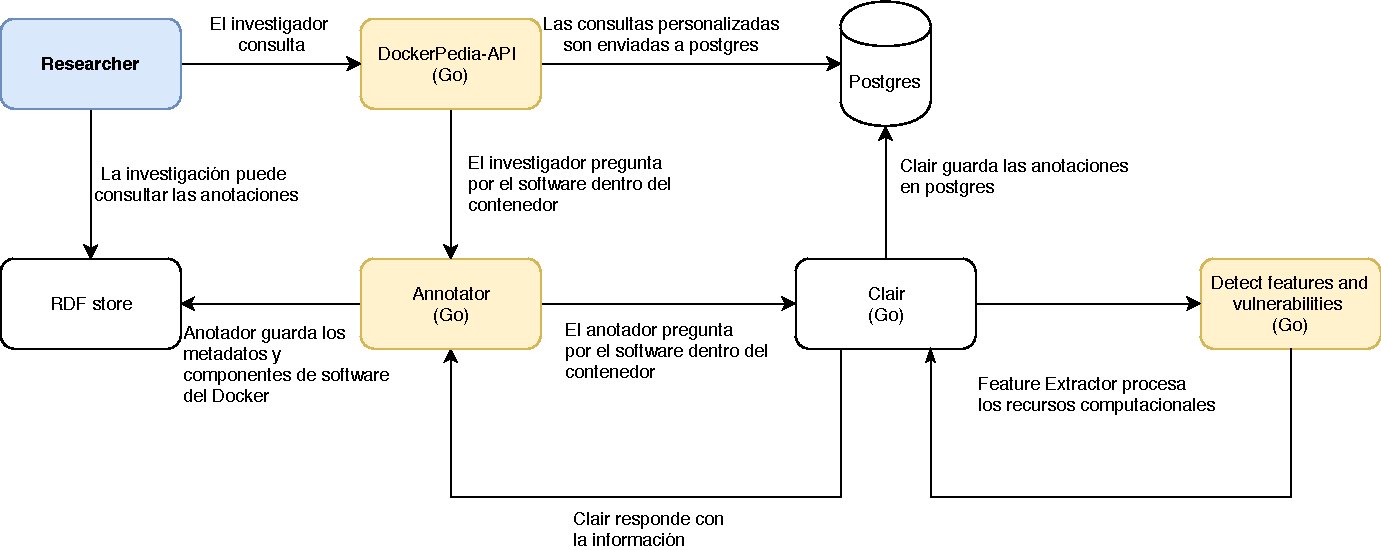
\includegraphics[width=\textwidth]{Figures/arch.pdf}
\caption{Figure caption.}\label{fig:arch}
\end{figure*}


\begin{enumerate}
    \item El investigador pregunta sobre la información de la imagen al sistema de anotación de DockerPedia. Este microservicio se encuentra escrito en GO y disponible en \href{\url{}}
    \item 
     The researcher asks about the information of an image to DockerPedia annotator. DockerPedia-API is written on GoLang.
    \item Annotator asks the software and vulnerabilities inside the image to Clair using the API. We use a own custom Clair version that also can detect Software Components installed by Conda. DockerPedia-Annotator and Clair are written on GoLang.
    \item To obtain the building steps, labels, architectue and more information.  Annotator gets the manifest of the image from DockerHub. 
    \item Annotator stores the information using RDF and the proposed ontology. 
\end{enumerate}


\section{Resultados y discusión}\label{s5.4}

\subsection{Reproducibilidad}
\todo[inline]{compare the outputs: soykb}
\todo[inline]{compare the outputs: epigenomics}
%the resulting image (0.1 degree image of the sky) against the one generated by the baseline execution, obtaining a similarity factor of 1.0 (over 1.0) with a threshold of 0.85. In the Epigenomics and SoyKB workflows, the output data is non-deterministic due to the existence of probabilistic steps. In this case, the use of a hash method is unfeasible. Hence, we validated the correct execution of the workflow by checking that correct output files were actually produced, and that the standard errors produced by the applications did not contain any error message. In both cases the results obtained in each infrastructure were equivalent in terms of their size (e.g., number of lines) and content.
\todo[inline]{compare the outputs: internal extinction}

%todo: Results show that the VM execution environments deployed by all scripts are able to fully execute their related workflows. To check that not only the workflows are successfully executed but also that the results are correct and equivalent, we checked their produced output data. In the case of Montage, which produces an image as output, we used a perceptual hash tool20 to compare


\subsection{Similitud y diferencias}

\subsection{Uso de disco }
%To evaluate that the Docker Images are lightweight and storable, we built two images, one using Docker, the other using virtual machines using WICUS~\cite{santana2017reproducibility} and we compared the disk usage of both.

Los resultados sobre la comparación de uso de disco muestra que existe una disminución de 64\%. La tabla \ref{storage-reduce} muestra la diferencia para el sistema de workflow Pegasus y dispel4py.

\begin{table}[]
\begin{tabular}{|l|l|l|}
\hline
Approach       & Pegasus (MB) & dispel4py \\ \hline
Virtualization & 1929         & -  \\ \hline
Container      & 690          &  - \\ \hline
\end{tabular}
\caption{Disk usage pegasus and dispel4py images.}
\label{storage-reduce}
\end{table}


